\documentclass[11pt]{article}

\usepackage[margin=1in]{geometry}
\usepackage{booktabs}
\usepackage{amsmath}
\usepackage{graphicx}
\usepackage{xcolor}
\usepackage{titlesec}
\usepackage[hidelinks]{hyperref}
\usepackage{parskip}

\definecolor{linknavy}{RGB}{20,40,90}
\hypersetup{colorlinks=true, urlcolor=linknavy, linkcolor=linknavy}
\titleformat{\section}{\large\bfseries}{\thesection}{0.6em}{}
\titlespacing{\section}{0pt}{1.3em}{0.4em}
\newcommand{\code}[1]{\texttt{\small #1}}

\title{\vspace{-2em}\textbf{diffusion-tinker: reproduction results}}
\author{Srijit Iyer}
\date{July 2026}

\begin{document}
\maketitle
\vspace{-1.5em}

\noindent\textbf{diffusion-tinker} is a TRL-style library for RL post-training of diffusion models: you give it a model, a reward, and a set of prompts, and it runs one of six algorithms (FlowGRPO, DDRL, DRaFT, DiffusionDPO, DDPO, SFT) behind a single \code{Trainer}/\code{Config} API on top of HuggingFace \code{diffusers}. It targets Stable Diffusion 3.5 and FLUX.1.

This note collects the reproduction results. Every number is from a real run on the Stanford cluster (A5000 24\,GB, or A6000-Ada 48\,GB for FLUX), LoRA rank 16, bf16. The implementations were verified at the level of gradients-reaching-weights and correct pixel ranges first; Appendix~\ref{app:verify} lists what that turned up.

\section{The main finding}

The single most useful result is about when RL helps at all: \textbf{an RL reward goes up when the base model has room to improve on it, and stays flat when the model is already near that reward's ceiling.} This is a property of the reward/model pairing, not a bug or a tuning failure, and it explains the rest of this note.

Rewards with headroom climb: OCR (to 1.00), object counting (0.79 to $\sim$1.0), CLIP-score (27 to 29), aesthetic under DRaFT (5.9 to 9.6). Rewards SD3.5 is already good at stay flat: PickScore ($\sim$22.5) and HPS-v2 ($\sim$0.28) do not move, because there is nothing to push up. So the earlier puzzle of PickScore ``not working'' was really PickScore being the wrong reward to show a gain on.

\section{Results}

\begin{center}
\begin{tabular}{@{}llll@{}}
\toprule
\textbf{Trainer} & \textbf{Task / reward} & \textbf{Result} & \textbf{Status} \\
\midrule
FlowGRPO     & OCR, counting, CLIP       & OCR 1.00; count 0.79$\to$1.0; CLIP 27$\to$29 & validated \\
DRaFT        & aesthetic (LAION)         & 5.9 $\rightarrow$ 9.6            & validated \\
DiffusionDPO & preference pairs          & winner/loser separation learned & validated \\
SFT          & Naruto denoising          & flow-matching loss converges    & validated \\
DDRL         & counting/OCR + data anchor & climbs with anchor, collapses without (\S\ref{sec:grid}) & validated w/ anchor \\
DDPO/DPOK    & counting, OCR             & ratio $\sim$1.0, but reward does not reliably climb & tested, weak \\
\bottomrule
\end{tabular}
\end{center}

DDPO is the one trainer that does not reliably move a reward, even on an easy headroom task with the fixed setup (counting degraded 0.34\,$\to$\,0.10, OCR net-flat). This is an algorithmic limit, PPO without GRPO's group-relative advantage, not a code bug: the ratio is corrected and gradients reach the weights.

\section{Comprehensive grid: algorithm $\times$ anchor $\times$ reward}
\label{sec:grid}

The rigorous comparison: FlowGRPO vs DDRL, each at anchor strength $\beta \in \{0,\text{mid},\text{high}\}$, on two headroom rewards (counting, OCR), matched budget (group 12, 20 rollout steps, noise 0.1, lr $10^{-4}$).

\begin{figure}[h]
\centering
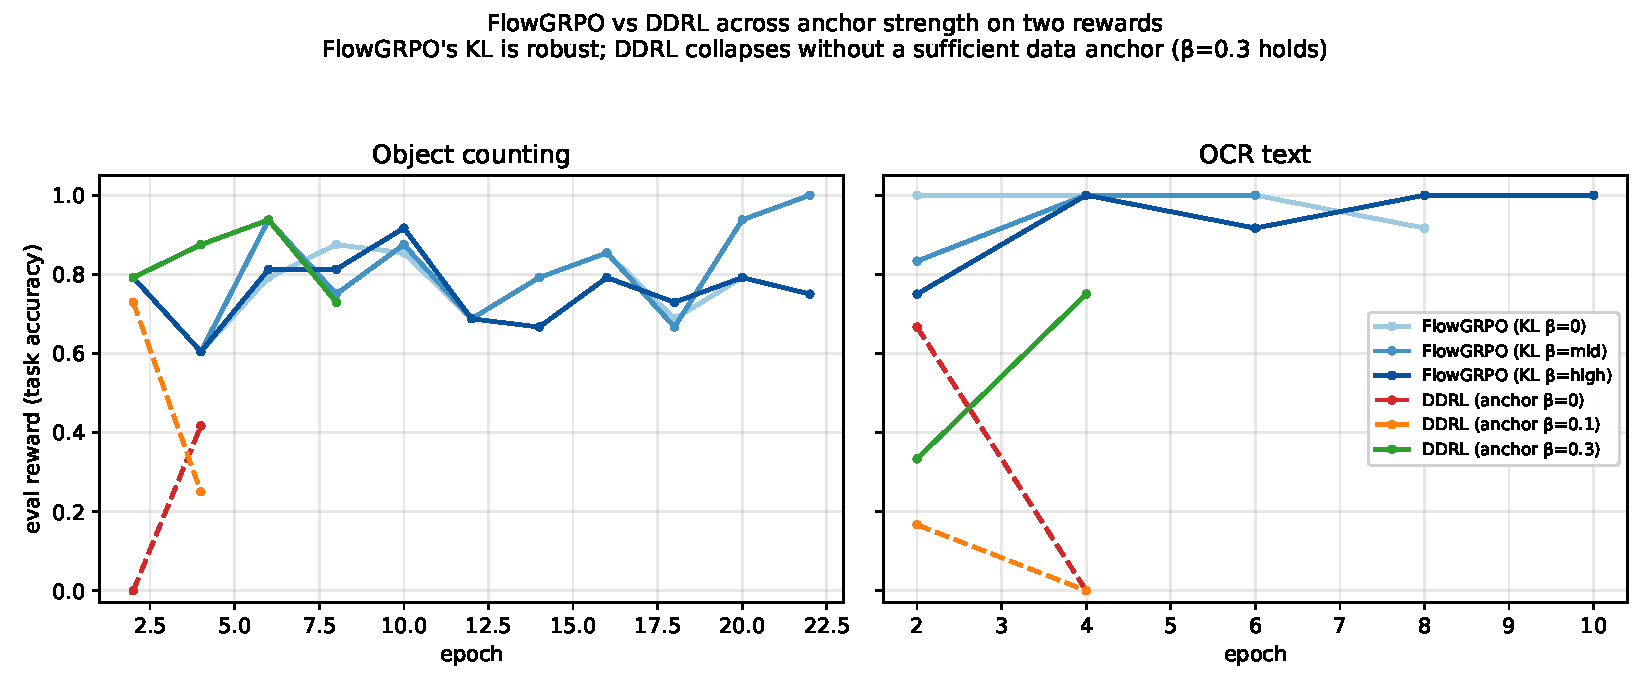
\includegraphics[width=\textwidth]{figures/grid_comparison.pdf}
\caption{FlowGRPO's KL anchor is robust: it climbs or holds high at every $\beta$, on both rewards, and never collapses. DDRL collapses without an anchor ($\beta=0$, red) as expected; a stronger anchor ($\beta=0.3$, green) lets it climb first but only \emph{delays} the collapse, on OCR it reaches 1.0 then crashes back to 0.25. So the data anchor is real but weaker than the KL, and needs a larger $\beta$ (or a task-matched anchor set) to hold the whole run.}
\label{fig:grid}
\end{figure}

This confirms the anchor intuition directionally, no anchor collapses and an anchor lets the run survive and climb, while being honest that $\beta=0.3$ delays collapse rather than preventing it.

\section{Reward increase on a headroom task}

The clearest single demonstration that RL raises a reward when there is room: FlowGRPO on an object-counting reward, does the image contain the right number of objects, scored with an open-vocabulary detector.

\begin{figure}[h]
\centering
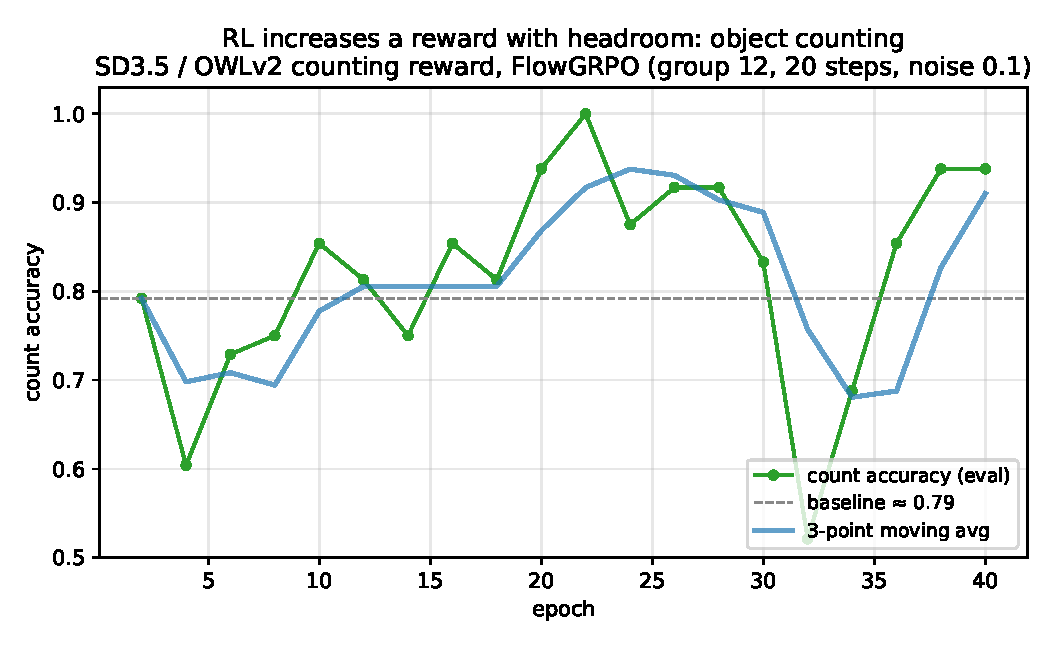
\includegraphics[width=0.75\textwidth]{figures/count_climb.pdf}
\caption{Count accuracy climbs from $\sim$0.79 to a peak of 1.0 and holds near 0.9. A practical lesson: a detector-based reward needs coherent rollout images, so it needs more sampling steps and less exploration noise than PickScore does, otherwise the detector finds nothing and the reward is flat zero. There is a genuine tension between exploration noise for the RL and clean images for a strict reward.}
\label{fig:count}
\end{figure}

\section{FLUX.1-schnell}

The FLUX code path (auto-detection, packed latents, sampling/replay log-probs, schnell guidance, decode) runs end-to-end with FlowGRPO + aesthetic on the 48\,GB card. Convergence is modest and noisy: schnell is a four-step \emph{distilled} model not built for stochastic SDE sampling, and its importance ratio sits near 0.92 vs $\sim$1.0 on SD3. Status: code path validated on FLUX, convergence weak on schnell. FLUX.1-dev (non-distilled) is the better RL target and has not been run.

\section{Limitations}

Eval curves use a small number of prompts and are noisy, read the trend, not any single point. DDPO does not reliably improve rewards. DDRL's anchor at $\beta=0.3$ delays but does not fully prevent collapse. DiffusionDPO's re-run is currently blocked by Pick-a-Pic HF dataset gating. FLUX.1-dev is unrun.

\appendix
\section{Verification}
\label{app:verify}

The runs above are on code that was corrected first. The library had a passing test suite and clean smoke runs, but several trainers were not learning, because a smoke test that produces an image and a reward says nothing about whether gradients reach the weights or whether the reward is even moving. Checking directly turned up:

\begin{itemize}
\setlength{\itemsep}{1pt}
\item \textbf{One optimizer step per epoch.} The RL trainers folded a whole batch into a single update, so a long run did only a few dozen steps. Stepping per mini-batch is what actually let the reward move.
\item \textbf{Importance-ratio bias.} Training the final near-zero-noise denoising step made the sampling-vs-replay ratio $\sim$0.92 instead of 1.0; dropping that step fixed it. Separately, sampling ran without autocast while replay ran with it, biasing the ratio, fixed by aligning precision.
\item \textbf{DRaFT never trained.} A no-grad warmup populated \code{autocast}'s weight cache with detached bf16 casts of the LoRA weights, which the gradient loop reused, so every LoRA gradient came back \code{None}. Fixed with \code{cache\_enabled=False} (reward then 5.9\,$\to$\,9.6).
\item \textbf{VAE range, both directions.} Decode clamped $[-1,1]$ straight to $[0,1]$ (55\% of every image crushed to black); encode fed $[0,1]$ to a VAE expecting $[-1,1]$.
\item \textbf{Memory.} The rollout trajectory was kept alive into the next epoch's sampling (doubling peak memory) and the VAE decoded a whole sample group at once; freed per epoch and chunked the decode. Plus smaller fixes to the PEFT adapter API, the reward-model APIs across \code{transformers} versions, and the noise/KL interaction (low noise inflates the KL penalty $\sim 1/\text{noise}^2$, silently freezing the policy).
\end{itemize}

\noindent Because the earlier ``validated'' numbers were measured on broken images and latents, every result here is a fresh run on the fixed code. Source and per-run logs: \url{https://github.com/srijitiyer/diffusion-tinker}.

\end{document}
